\documentclass[border=4pt,12pt]{standalone}
% House style for redrawn exam diagrams (diagram-v4: 0.4pt lines, filled -latex arrows, fine dashes; stipple and hatching drawn as real dots/lines (no PDF/SVG patterns, so they render in every browser and at any scale); transparent background). Every figure \input's this.
\usepackage{amsmath,amssymb}
\usepackage{txfonts}
\usepackage{pdfrender,xcolor}
% \halo{text}: label on shading. The shading stops just around each letter's outline (a thin knock-out that follows the
% glyphs, like the papers' typesetting), never a box. Owner: "I don't want a box around the text".
\newcommand{\halo}[1]{\leavevmode\rlap{\pdfrender{TextRenderingMode=2,LineWidth=2.2pt,LineJoinStyle=1,StrokeColor=white,FillColor=white}#1}#1}
\usepackage{tikz,pgfplots}
\pgfplotsset{compat=1.18}
\usetikzlibrary{arrows.meta,calc,angles,quotes,patterns,patterns.meta,intersections,positioning,decorations.markings,shapes.geometric}
% Stipple and hatching are drawn as actual dots / lines clipped to the region (path picture), NOT as pattern fills:
% SVG <pattern> fills vanish or blur when browsers scale the image, so the owner could not see the shading.
% Each dot is a 0.72pt square (keeps SVGs small; reads as a dot at print size). Dots sit on one global staggered grid, so neighbouring regions line up.
\makeatletter
\newdimen\ex@x \newdimen\ex@y \newdimen\ex@xa \newdimen\ex@ya \newdimen\ex@xb \newdimen\ex@yb \newcount\ex@row
\def\exam@stipplecolor{black!75}\def\exam@dotr{0.42pt}\def\exam@dotgap{2.5}
\def\ex@rowdots{\ifdim\ex@x<\ex@xb \pgfpathrectangle{\pgfqpoint{\dimexpr\ex@x-0.36pt\relax}{\dimexpr\ex@y-0.36pt\relax}}{\pgfqpoint{0.72pt}{0.72pt}}\advance\ex@x by \exam@dotgap pt\relax\expandafter\ex@rowdots\fi}
\def\exam@stipple{%
  \pgftransformreset% dots are sized in real points even inside scaled pictures
  \pgfpointanchor{path picture bounding box}{south west}\ex@xa=\pgf@x \ex@ya=\pgf@y
  \pgfpointanchor{path picture bounding box}{north east}\ex@xb=\pgf@x \ex@yb=\pgf@y
  \pgfsetfillcolor{\exam@stipplecolor}\pgfmathsetmacro\ex@h{\exam@dotgap/2}%
  \pgfmathtruncatemacro\ex@r{floor(\ex@ya/\ex@h)-1}\ex@row=\ex@r\relax
  \ex@y=\ex@r\dimexpr\ex@h pt\relax
  \loop\ifdim\ex@y<\ex@yb
    \pgfmathtruncatemacro\ex@c{floor(\ex@xa/\exam@dotgap)-1}\ex@x=\ex@c\dimexpr\exam@dotgap pt\relax
    \ifodd\ex@row \advance\ex@x by \ex@h pt\fi
    \ex@rowdots
    \advance\ex@y by \ex@h pt \advance\ex@row by 1
    \ifnum\numexpr\ex@row-(\ex@row/4)*4\relax=0 \pgfusepath{fill}\fi% flush every 4 rows: bounded TeX memory, few clip copies in the SVG
  \repeat\pgfusepath{fill}}
\newdimen\ex@d
\def\exam@hatch#1{% #1 = 1 for /, -1 for \ ; lines 45 degrees, 3pt apart
  \pgftransformreset
  \pgfpointanchor{path picture bounding box}{south west}\ex@xa=\pgf@x \ex@ya=\pgf@y
  \pgfpointanchor{path picture bounding box}{north east}\ex@xb=\pgf@x \ex@yb=\pgf@y
  \ex@d=\dimexpr\ex@yb-\ex@ya\relax \ex@x=\dimexpr\ex@xa-\ex@d\relax
  \loop\ifdim\ex@x<\ex@xb
    \ifnum#1>0 \pgfpathmoveto{\pgfqpoint{\ex@x}{\ex@ya}}\pgfpathlineto{\pgfqpoint{\dimexpr\ex@x+\ex@d\relax}{\ex@yb}}%
    \else \pgfpathmoveto{\pgfqpoint{\ex@x}{\ex@yb}}\pgfpathlineto{\pgfqpoint{\dimexpr\ex@x+\ex@d\relax}{\ex@ya}}\fi
    \advance\ex@x by 4.24pt
  \repeat
  \pgfsetlinewidth{0.4pt}\pgfsetstrokecolor{black}\pgfusepath{stroke}}
\def\examstipple{\exam@stipple}\def\examhatch{\exam@hatch}\def\examsetstipplecolor#1{\def\exam@stipplecolor{#1}}\def\examsetdotgap#1{\def\exam@dotgap{#1}}
\makeatother
% (legacy pattern kept for old files)
% staggered stipple like the NESA papers' dotted shading
\pgfdeclarepatternformonly{exam stipple}{\pgfpointorigin}{\pgfqpoint{2.2pt}{2.2pt}}{\pgfqpoint{2.2pt}{2.2pt}}{%
  \pgfpathcircle{\pgfqpoint{0.55pt}{0.55pt}}{0.42pt}\pgfpathcircle{\pgfqpoint{1.65pt}{1.65pt}}{0.42pt}\pgfusepath{fill}}
\tikzset{
  every picture/.style={line width=0.6pt, >={Latex[length=2mm,width=1.3mm]}},
  curve/.style={line width=0.6pt},
  open arrow/.style={-{Latex[length=2mm,width=1.3mm]}},  % owner: filled -latex heads everywhere, no open chevrons
  aux/.style={dash pattern=on 2pt off 1.5pt, line width=0.6pt},
  shade/.code={\def\exA{#1}\def\exB{none}\ifx\exA\exB\else\pgfkeysalso{fill=black!18}\fi},
  shade/.default=on,
  shade dots/.style={fill=none, path picture={\examstipple}},
  stipple color/.code={\examsetstipplecolor{#1}},
  stipple gap/.code={\examsetdotgap{#1}},
  shade dense dots/.style={fill=none, stipple gap=1.6, path picture={\examstipple}},
  shade hatch/.style={fill=none, path picture={\examhatch{1}}},
  shade hatch reverse/.style={fill=none, path picture={\examhatch{-1}}},
  shade solid/.style={fill=black},
  pt/.style={circle, fill, inner sep=1.1pt},
  open pt/.style={circle, draw, fill=white, inner sep=1.1pt},
}
\pgfplotsset{
  exam axes/.style={axis lines=middle, axis line style={->}, xlabel={$x$}, ylabel={$y$},
    xlabel style={anchor=west}, ylabel style={anchor=south}, tick label style={font=\small},
    every axis plot/.append style={line width=0.6pt, black}, samples=200, clip=false,
    enlargelimits=false, axis on top},
}

\begin{document}
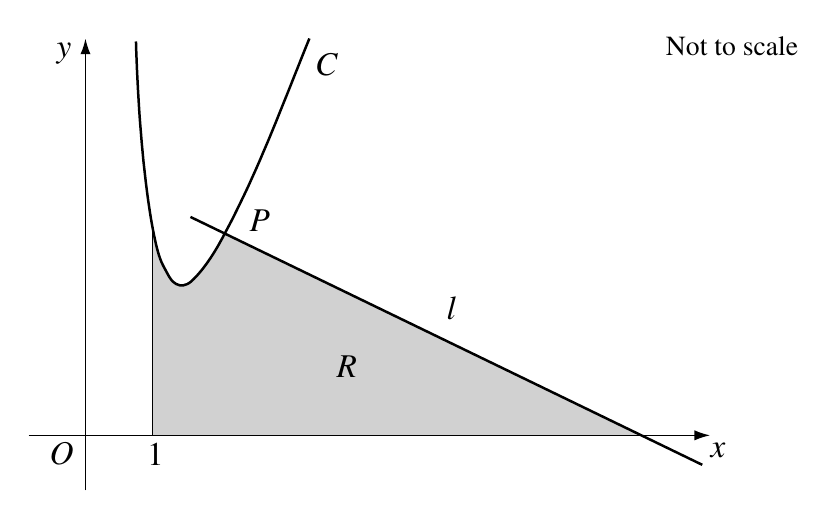
\begin{tikzpicture}[x=0.0127cm,y=-0.0127cm,font=\large]
  \path[shade] (134,203) -- plot[smooth] coordinates {(134,203) (134.4,205.5) (134.9,208) (135.4,210.6) (135.9,213.1) (136.5,215.6) (137,218.1) (137.6,220.6) (138.2,223.1) (138.8,225.6) (139.5,228.1) (140.1,230.5) (140.8,233) (141.5,235.3) (142.3,237.5) (143.1,239.6) (144.1,241.6) (145.2,243.6) (146.5,245.7) (147.9,247.8) (149.1,249.9) (150.3,252.2) (151.5,254.2) (152.8,256.1) (154.1,257.7) (155.4,259.1) (156.9,260.3) (158.4,261.2) (159.9,261.8) (161.5,262.1) (163.1,262.2) (164.8,262) (166.6,261.5) (168.4,260.8) (170.2,259.8) (172,258.5) (173.8,257.1) (175.5,255.6) (177.2,254) (178.8,252.2) (180.4,250.4) (181.9,248.5) (183.4,246.6) (185,244.5) (186.4,242.5) (187.9,240.4) (189.4,238.3) (190.8,236.2) (192.3,234) (193.8,231.8) (195.2,229.7) (196.7,227.6) (198,225.5) (199.4,223.3) (200.7,221.2) (201.9,219.1) (203,216.9) (204.1,214.7) (205.1,212.5) (206,210.3)} -- (623,412) -- (134,412) -- cycle;
  \draw[->] (10,412) -- (692,412);
  \draw[->] (67,467) -- (67,15);
  \draw (134,412) -- (134,203);
  \draw[line width=0.9pt] plot[smooth] coordinates {(117.5,18) (117.8,28.07) (118.2,38) (118.6,47.94) (119.1,57.87) (119.6,67.67) (120.2,77.61) (120.8,87.54) (121.5,97.47) (122.3,107.3) (123.1,117.2) (124,127.1) (124.9,136.8) (126,146.7) (127.1,156.5) (128.3,166.3) (129.6,176.1) (131,185.6) (132.5,195.2) (134.2,204.7) (136.1,214.2) (138.2,223.5) (140.5,231.8) (143.2,239.1) (147,246.5) (151.1,253.9) (154.4,258.2) (157.7,260.6) (161.3,261.9) (165,261.9) (168.8,260.7) (172.8,258) (178.3,252.5) (183.9,245.9) (189.2,238.8) (194.3,231.2) (199.1,223.3) (203.8,214.9) (208.3,206.4) (212.9,197.7) (217.3,188.9) (221.6,180.1) (225.9,171.2) (230.1,162.3) (234.1,153.4) (238.2,144.3) (242.1,135.3) (246,126.1) (249.9,117) (253.7,107.8) (257.5,98.59) (261.2,89.37) (264.9,80.14) (268.7,70.77) (272.4,61.53) (276.1,52.16) (279.8,42.92) (283.5,33.56) (287.2,24.34) (291,15)};
  \draw[line width=0.9pt] (172,193.5) -- (684,441.5);
  \node at (45.5,30) {$y$};
  \node at (309,41.5) {$C$};
  \node at (241,197) {$P$};
  \node at (433,285.5) {$l$};
  \node at (328.5,343.5) {$R$};
  \node at (43,431) {$O$};
  \node at (137,431) {$1$};
  \node at (699,427) {$x$};
  \node[anchor=east,font=\normalsize] at (790,23) {Not to scale};
\end{tikzpicture}
\end{document}
